\documentclass{standalone}
\usepackage{tikz}
\usepackage{ctex,siunitx}
\usepackage{tkz-euclide}
\usepackage{amsmath}
\usetikzlibrary{patterns, calc}
\usetikzlibrary {decorations.pathmorphing, decorations.pathreplacing, decorations.shapes,}
\begin{document}
\small
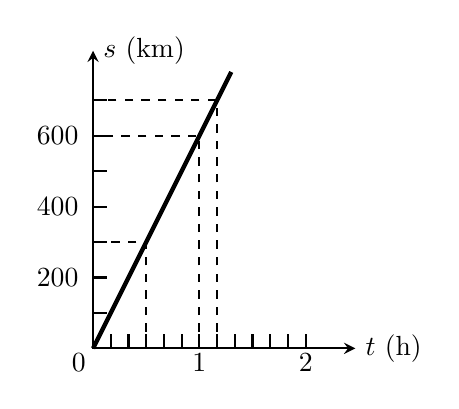
\begin{tikzpicture}[>=stealth, thick,scale=0.9]
  \draw [<->](0,4.2)node[right]{$s$ (\unit{km})}--(0,0)--(3.7,0)node[right]{$t$ (\unit{h})};
  \foreach \x in {1,2,3,...,12}
  {
      \draw(\x/4, 0) --(\x/4, .2);
  }
  \foreach \y in {1,2,3,...,7}
  {
      \draw(0,\y/2)--(.2, \y/2);
  }
  \node at (-.2,-.2){$0$};
  \node at (1.5,-.2){$1$};
  \node at (3,-.2){$2$};
  \node at (-.5,1){$200$};
  \node at (-.5,2){$400$};
  \node at (-.5,3){$600$};
  \draw [dashed] (1.5/2,0)--(1.5/2,1.5)--(0,1.5);
  \draw [dashed] (1.5,0)--(1.5,3)--(0,3);
  \draw [dashed] (1.5+1.5/6,0)--(1.5+1.5/6,3.5)--(0,3.5);
  \draw[ultra thick](0,0)--(1.3*1.5,3.9);
\end{tikzpicture}
\end{document}